%\documentclass[landscape,20pt]{extarticle}
%\usepackage{eso-pic,graphicx}
%\usepackage{bbm}
%\usepackage{amssymb,amsmath,verbatim,stmaryrd}
%\usepackage{amsthm}
%\usepackage{pgf,tikz,yhmath}
%\usepackage{ifthen}
%\usetikzlibrary{arrows}
%\usepackage[T1]{fontenc}
%\usepackage[french]{babel}
%\usepackage[utf8]{inputenc}
%\usepackage{palatino,eulervm}

%\addtolength{\hoffset}{-0.15cm}
%\textwidth 228mm 
%\oddsidemargin+0.4cm \evensidemargin -0.8cm

%\newcommand\BackgroundPic{
%\put(0,0){
%\parbox[b][\paperheight]{\paperwidth}{%
%\vfill
%\centering
%\includegraphics[width=\paperwidth,height=\paperheight]{muraille.jpg}
%\vfill
%}}}

%\pagestyle{empty}

%\makeatletter
%\newcounter{exo}[subsection]
%\newenvironment{exo}[2][]
%  {\edef\@exer{#1}%
%   \ifx  \@exer\empty{} \else{\setcounter{exo}{#1}\addtocounter{exo}{-1}}\fi%%
%   \refstepcounter{exo}
%   { \center \bf \large{Exercice \theexo #2} \\ \bigskip \bigskip }%
   %
%   }
%  {\pagebreak}
%\makeatother

%\newcommand{\N}{\mathbb{N}}
%\newcommand{\Z}{\mathbb{Z}}
%\newcommand{\Q}{\mathbb{Q}}
%\newcommand{\R}{\mathbb{R}}
%\newcommand{\C}{\mathbb{C}}


% \begin{document}


%\AddToShipoutPicture{\BackgroundPic}

% Exercices collège: 1 \`a 42
%Il en faut 24

% Exercices  lycée:: 42 \`a 96
%Il en faut 11

% Exercices olympiques: 97 à 142
%Il en faut 9


\newcommand{\nstar}[1]
{
  \ifthenelse{\equal{#1}{0}}{}{}
  \ifthenelse{\equal{#1}{1}}{\mbox{ }$^ {\star}$}{}
  \ifthenelse{\equal{#1}{2}}{\mbox{ }$^ {\star \star}$}{}
  \ifthenelse{\equal{#1}{3}}{\mbox{ }$^ {\star \star \star}$}{}
  \ifthenelse{\equal{#1}{4}}{\mbox{ }$^ {\star \star \star \star}$}{}
  \ifthenelse{\equal{#1}{5}}{\mbox{ }$^ {\star \star \star \star \star}$}{}
  \ifthenelse{\equal{#1}{6}}{\mbox{ }$^ {\star \star \star \star \star \star}$}{}
  \ifthenelse{\equal{#1}{7}}{\mbox{ }$^ {\star \star \star \star \star \star \star}$}{}
  \ifthenelse{\equal{#1}{8}}{\mbox{ }$^ {\star\star \star \star \star \star \star \star}$}{}
}

%%%%%%%%%%%% EXERCICES COLLEGE


\begin{exo}{\nstar{2}}
Trouver tous les entiers $n$ strictement positifs tels que $2^n+n$ divise $8^n+n$.
\medskip
\textit{Elliot Thorel}

\end{exo}

%2
%Théodore Fougereux
\begin{exo}{}
On écrit les fractions $\dfrac{1}{2},\dfrac{2}{3},...,\dfrac{n-1}{n}$ au tableau. On s'autorise à "\textit{retourner}" certaines fractions, \textit{retourner} une fraction consiste à remplacer $\dfrac{a}{b}$ par $\dfrac{b}{a}$. Trouver les $n$ tels qu'on puisse \textit{retourner} certaines fractions de sorte à ce que le produit des nombres au tableau soit $1$.
\end{exo}


%3
%%Mathieu Barré
\begin{exo}{\nstar{4}}
Soit $ABC$ un triangle équilatéral et $P$ un point à l'intérieur de ce triangle. Soient $D,E$ et $F$ les pieds des perpendiculaires de $P$ sur $[BC],[CA]$ et $[AB]$ respectivement. Montrer que:
\begin{enumerate}
\item $AF+BD+CE=AE+BF+CD$ et que
\item $|APF|+|BPD|+|CPE|=|APE|+|BPF|+|CPD|$,
\end{enumerate}
où $|XYZ|$ désigne l'aire du triangle $XYZ$.
\end{exo}

%4
%Giancarlo
\begin{exo}{\nstar{3}}
Soient $x,y$ deux entiers relatifs et $p$ un nombre premier. Montrer que si l'on a $x\equiv y \ [p]$ , alors on a $x^p\equiv y^p \ [p^2]$.

\medskip
\textit{Elliot Thorel}
\end{exo}

%5
%Rémi
\begin{exo}{\nstar{2}}
Trouver tous les quadruplets d'entiers positifs $(w,x,y,z)$ tels que
$$w^x+w^y=w^z.$$
\medskip
\textit{Adam Donadille et Antoine Corbineau}

\end{exo}

%6
%Raphael Ducatez
\begin{exo}{}
En notant $a,b,c$ les trois solutions réelles de l'équation $x^3-2x^2-5x+6=0$, combien vaut $\dfrac{1}{ab}+\dfrac{1}{ac}+\dfrac{1}{bc}$?

\medskip
\textit{Anatole Bouton}
\end{exo}




%7
%Raphael
\begin{exo}{}
Quel est le chiffre des unités de $1!+2!+...+42!$ ?

\medskip
\textit{Anatole Bouton}
\end{exo}


%Mathieu Barré
%8
\begin{exo}{\nstar{4}}
Trouver tous les entiers relatifs $x$ et $y$ tels que \[x^2y+7x=x^2+3xy+3y+4.\]

\medskip
\textit{Elliot Thorel, Augutin Kheng et Camille Ordenneau}
\end{exo}

%9
%Mathieu Barré
\begin{exo}{\nstar{3}}
Les nombres de $1$ à $n$ sont écrits au tableau. \`A chaque étape, on choisit deux nombres $a$ et $b$ distincts du tableau, on les efface puis on les remplace par $ab+a+b$, et on réitère ce processus. Quel sera le dernier nombre écrit au tableau ?
%vide

\medskip
\textit{Adam Donadille}
\end{exo}

%10
\begin{exo}{\nstar{6}}Soit $[EF]$ un segment inclus dans le segment $[BC]$ tel que le demi-cercle de diamètre $[EF]$ est tangent à $[AB]$ en $Q$ et à $[AC]$ en $P$. Prouver que le point d'intersection $K$ des droites $(EP)$ et $(FQ)$ appartient à la hauteur issue de $A$ du triangle $ABC$.
\end{exo}

%11
%Mathieu Barré
\begin{exo}{\nstar{3}}
Soient $a$ et $b$ deux nombres réels et $f$ la fonction de $\mathbb{R}$ dans $\mathbb{R}$ qui à $x$ associe $x^2+ax+b$. On suppose  qu'il existe un réel $t$ tel que $f(t)=f(f(f(t)))=0$. Montrer que $f(0) \times f(1)=0$.

\medskip
\textit{Anatole Bouton}
\end{exo}

%12
%Mathieu Barré
\begin{exo}{\nstar{3}}
Combien y a-t-il d'entiers positifs $n$ tels que
\[\frac{n^{2016}}{n-2016}\]
soit un nombre entier ?
\end{exo}

%13
%Raphael
\begin{exo}{}
Quel est le rapport entre l'aire d'un carré circonscrit à un cercle et l'aire d'un carré inscrit dans le même cercle?

\medskip
\textit{Anatole Bouton et Gaetan Dautzenberg}
\end{exo}

%14
% Andrei Barbu
\begin{exo}{}
On considère $2019$ nains en ligne numérotés $1,2,...,2019$. Chaque nain possède une pomme rouge ou verte sur sa tête et voit les pommes de tous les nains qui ont un plus petit numéro (donc le nain $i$ voit le nain $j$ si et seulement si $i>j$). Blanche Neige demande à chaque nain quelle est la couleur de sa pomme. Elle commence par demander au nain $2019$, puis au nain $2018$, et ainsi de suite jusqu'au nain $1$. Si le nain dit la bonne couleur, il peut manger sa pomme. Si les nains se mettent d'accord au début, quel est le plus grand nombre de pommes qu'ils peuvent s'assurer de manger au total?

\medskip
\textit{Anatole Bouton}

\end{exo}

%Gabriel
%15
\begin{exo}{\nstar{4}}
Montrer que tous les termes de la suite $\left(a_{n}\right)$ définie par
\[\begin{cases}
a_{1}=a_{2}=a_{3}=1\\
a_{n+1}=\frac{1+a_{n-1}a_{n}}{a_{n-2}}
\end{cases}\]
sont des entiers.
\end{exo}

%16
%Mathieu Barré
\begin{exo}{\nstar{3}}
On considère $101$ points, placés à l'intérieur d'un carré $10\times10$. Montrer qu'il existe un triangle parmi les $101$ points avec une aire inférieure ou égale à $1$.

\medskip
\textit{Elliot Thorel}
\end{exo}

%Gabriel
%17
\begin{exo}{\nstar{4}}
 Existe-t-il une
suite $\left(u_{n}\right)_{n \geq 1}$ d'entiers naturels non nuls telle que pour tous entiers $m,n \geq 1$
$u_{n}$ et $u_{m}$ sont premiers entre eux si et seulement si $\left|n-m\right|=1$
?

\medskip
\textit{Adam Donadille}
\end{exo}

%18
%Mathieu
\begin{exo}{\nstar{3}}
Soit $ABC$ un triangle isocèle en $A$ et $D$ le pied de la bissectrice intérieure issue de $B$. On suppose que $BC=AD+DB$. Combien vaut $\widehat{BAC}$ ?
\end{exo}

%19
%Mathieu
\begin{exo}{\nstar{3}}
$20$ enfants sont attendus par leurs grands-pères à la sortie de l’école primaire.
On suppose que deux enfants quelconques choisis parmi les $20$ ont au moins un grand-père en commun.
Montrer qu’il y a au moins un grand-père qui attend au moins $14$ de ses petits-enfants.

\medskip
\textit{Elsa Lubek et Isaline Duperon}
\end{exo}

%Martin Rakovsky
%20
\begin{exo}{}
Trouver toutes les paires d'entiers naturels $(a,b)$ telles que :
$$ab+2=a^3+2b$$
\end{exo}

%21
%Martin Rakovsky
\begin{exo}{}
Trouver tous les nombres premiers distincts $p,q,r$ tels que:\\
$ p|qr-1$\\
$ q|pr-1$\\
$ r|pq-1$\\
\end{exo}

%22
%Guillaume
\begin{exo}{\nstar{2}}
On inscrit $100$ entiers sur un cercle. Leur somme vaut $1$. On appelle séquence positive une suite de nombres consécutifs sur le cercle telle que leur somme soit strictement positive. Combien y a-t-il de séquences positives sur le cercle ?
\end{exo}

%23
%Théodore Fougereux (AM-GM)
\begin{exo}{}
Trouver la valeur minimale de l'expression $S$ suivante:
$$S=\dfrac{a+b+c}{a^2+b^2+c^2+3}$$
Avec $a,b,c\in \mathbb{R}$.
\end{exo}

%24
%Martin Rakovsky
\begin{exo}{}
On considère deux entiers $m$ et $n$ et un nombre premier $p$ qui vérifient $0<m<n<p$. On suppose aussi que $p$ divise $m^2+1$ et $n^2+1$. Montrer que $p$ divise aussi $mn-1$.

\medskip
\textit{Anatole Bouton}
\end{exo}

%25
%Cécile
\begin{exo}{\nstar{3}}
Soit $ABCD,ECGF$ deux carrés tels que $B,C,G$ sont alignés et $A,D,E,F$ sont
du même côté de la droite $(BC)$. Soit $M$ l'autre point d'intersection des cercles
circonscrits à $ABCD$ et à $ECGF$.

Donner une autre construction du point $M$, n'utilisant qu'une règle non graduée.
\end{exo}



%26
%Savinien
\begin{exo}{\nstar{1}}
Un naturel $n$ est \emph{hydraté} s'il a exactement deux diviseurs premiers. Existe-t-il une suite de $18$ naturels consécutifs hydratés?

\medskip
\textit{Elsa Lubek et Isaline Duperon}
\end{exo}


%27
%Victor
\begin{exo}{\nstar{3}}
Alice et Bob jouent au jeu suivant:
Alice part du nombre $2$ et les joueurs jouent chacun leur tour.
A chaque tour, en notant $n$ le nombre atteint par le joueur précédent, on ajoute un nombre $m$ tel que $m$ divise $n$, $m \neq n$, et $m+n \leq 2016$.
Le premier joueur à ne plus pouvoir jouer a perdu.
Quel joueur peut s'assurer la victoire?
\end{exo}


%28
%Théo Lenoir
\begin{exo}{}
Soit $n$ un entier strictement positif. On dit qu'un sous ensemble $A$ de $\{1,2,...,n\}$ est "\textit{fade}" si pour tout $x,y$ dans $A$, $x+y$ n'est pas dans $A$. Selon la valeur de $n$, quel est le cardinal du plus grand ensemble \textit{fade} ?
\end{exo}


%29
%Guillaume
\begin{exo}{\nstar{2}}
Rusalka observe par un beau soir d'été $50$ étoiles. Avec son matériel d'astronomie, elle calcule la somme des distances mutuelles entre elles, qui vaut $S$. Soudain, un nuage surgit et cache $25$ étoiles. Montrer que la somme des distances mutuelles entre les $25$ étoiles restantes ne dépasse pas $S/2$.

\medskip
\textit{Elsa Lubek et Isaline Duperon}

\end{exo}


%30
%Vincent
\begin{exo}{ \nstar{3}}
Soit $f : \mathbb{R} \mapsto \mathbb{R}$ une fonction telle que $f(x+y) \geq f(xy)$ pour tous les réels $x$, $y$.
Montrer que $f$ est constante.

\medskip
\textit{Adam Donadille}
\end{exo}

%31
%Vincent
\begin{exo}{\nstar{3}}
Soit $ABC$ un triangle isocèle en $B$, puis $F$ un point sur la bissectrice de $\widehat{ABC}$ tel que $(AF)$ soit parallèle à $(BC)$.
Enfin, soit $E$ le milieu de $[BC]$, et soit $D$ le symétrique de $A$ par rapport à $F$.
Calculer le rapport des distances $EF / BD$.
\end{exo}

%32
\begin{exo}{\nstar{7}}
Soit $\mathcal{P}=A_1\ldots A_{2n}$ un $2n-$gone convexe dans le plan. Soit $P$ un point intérieur à $\mathcal{P}$, non situé sur une diagonale. Prouver que $P$ est contenu dans un nombre pair de triangles à sommets parmi les $A_i$.

\medskip
\textit{Elliot Thorel}
\end{exo}




%33
%Martin R
\begin{exo}{\nstar{1}}
Montrer que pour $x,y$ des réels positifs on a toujours:
$$\frac{x}{x^4+y^2}+\frac{y}{y^4+x^2}\leq \frac{1}{xy}$$

\medskip
\textit{Samuel Avril}
 \end{exo}

%34
%Eva
\begin{exo}{\nstar{2}}
Si tous les points du plan sont colorés soit en rouge, soit en orange soit en violet, peut-on toujours trouver deux points de même couleur éloignés d'un centimètre exactement ?
\end{exo}


%35
%Théo Lenoir
\begin{exo}{}
Soit $(a_n)_{n\in \mathbb{N}^*}$ une suite d'entiers strictement positifs tels que pour tout $i,j\ge 1$ entiers on ait:
$$pgcd(a_i,a_j)=pgcd(i,j)$$
Montrer que $a_i=i$ pour tout $i\ge 1$.
\end{exo}

%36
%Vincent
\begin{exo}{\nstar{3}}
Soit $ABC$ un triangle, $I$ le centre du cercle inscrit dans $ABC$, $D$ le pied de la hauteur de $ABI$ issue de $B$,
et $E$ le pied de la hauteur de $BCI$ issue de $B$.
Montrer que $AB = BC$ si et seulement si $BD = BE$.
\end{exo}

%37
%Savinien
\begin{exo}{\nstar{1}}
Pour quels entiers naturels $n\geq2$ peut-on assigner à chaque sommet d'un $2^n$-gone une suite de $n$ chiffres $0$ et $1$ de telle sorte que chaque suite soit utilisée une et une seule fois et que deux suites sur deux sommets adjacents diffèrent par exactement un chiffre? Ci-dessous, un exemple d'une telle configuration pour $n=3$.
\begin{center}
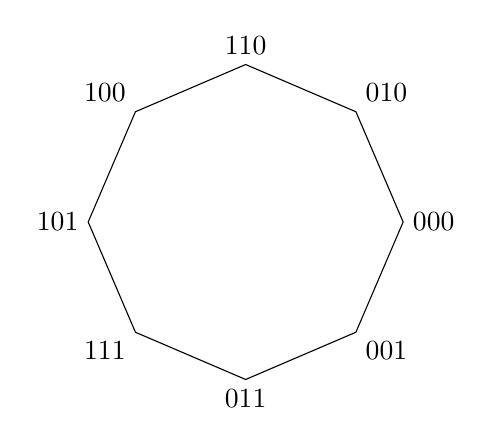
\begin{tikzpicture}
\draw(0,2)--(1.4,1.4)--(2,0)--(1.4,-1.4)--(0,-2)--(-1.4,-1.4)--(-2,0)--(-1.4,1.4)--(0,2);
\node[right] at (2,0){000};
\node[below right] at (1.4,-1.4){001};
\node[below] at (0,-2){011};
\node[below left] at (-1.4,-1.4){111};
\node[left] at (-2,0){101};
\node[above left] at (-1.4,1.4){100};
\node[above] at (0,2){110};
\node[above right] at (1.4,1.4){010};
\end{tikzpicture}
\end{center}

\medskip
\textit{Teiki Rigaud, Florian Chivé et Samuel Avril}
\end{exo}

%38
% Théodore Fougereux
\begin{exo}{}
On considère la suite $(a_n)_{n\in \mathbb{N}}$ définie par $a_0=2$ et $a_{n+1}=\sqrt{2a_n-1}$ pour tout $n\ge 0$.\\~~\\
$\bullet$ Montrer que $a_n$ est irrationel pour tout $n\ge 1$.\\~~\\
$\bullet$ La limite de $(a_n)$ est-elle irrationnelle (si elle existe)?
\end{exo}



%39
%Martin R.
\begin{exo}{\nstar{1}}
Soit $ABC$ un triangle actuangle. La bissectrice de $\widehat{BAC}$ coupe $BC$ en $D$ et le cercle circonscrit à $ABC$ en $E$. La tangente au cercle circonscrit à $ABC$ en $B$ coupe $AD$ en $F$. On suppose que $AD^2=2CD^2$. Montrer que $E$ est le milieu de $[AF]$.
 \end{exo}
 
 
%40
%Raphael
\begin{exo}{\nstar{1}}
On donne un nombre $n$ plus grand que $10^{2018}$.
Quel est le premier chiffre après la virgule dans l’écriture décimale de la racine carrée de $(n^2 +n+200)$ ?
 \end{exo}

%41
%Raphael
\begin{exo}{\nstar{1}}

Mathieu joue au billard sur un billard rectangulaire de
2,03 m sur 3,03 m. Sa boule, de 6 cm de diamètre, est
placée au milieu d’un grand côté du billard et Mathieu la
fait rouler, sans effet, selon un angle de 45 degré par rapport
au côté du billard.
En supposant que Mathieu lui ait donné suffisamment
de force, à quelle distance du point de départ le centre
de la boule sera-t-il au moment du 59e rebond ?

\end{exo}



%42
%Eva
\begin{exo}{\nstar{2}}
Eva et Victor disposent d'une tablette de chocolat rectangulaire de $n$ carrés de longueur et $2$ carrés de hauteur pour un certain entier $n>0$ et jouent au jeu suivant : chacun leur tour, en commençant par Eva, ils choisissent un carré de la tablette et le croquent ainsi que tous les carrés situés en haut ou à droite de celui-ci. Le dernier carré, en bas à gauche, étant fourré au piment, le joueur qui se trouve obligé de le manger a perdu. Est-ce que Victor ou Eva possède une stratégie gagnante ? Si oui, quelle est-elle ?

\medskip
\textit{Anatole Bouton}
\end{exo}


%%%%%%%%% Exos seconde-première %%%%%%%%%%%


%43
%Savinien
\begin{exo}{\nstar{1}}
Savinien et Martin jouent à un jeu. Les cases d'un échiquier $n\times n$ sont toutes vides et blanches, sauf celle en bas à gauche qui est noire et sur laquelle se trouve une tour. Tour à tour, Savinien et Martin la déplacent sur une case blanche et colorient cette case en noir (une tour peut se déplacer d'une case sur n'importe quelle autre case située sur la même ligne ou la même colonne). Le premier qui ne peut plus jouer a perdu. En fonction de $n$, qui a une stratégie gagnante et en quoi consiste-t-elle ?%Sur quelle case Savinien peut-il jouer son premier coup et avoir une stratégie gagnante?

\medskip
\textit{Raphaël Gandin}
\end{exo}

%Mathieu Barré
%44
\begin{exo}{}
Soit $q$ un entier strictement positif et $P$ un polynôme à coefficients entiers. Montrer qu'il existe un entier $n>0$ tel que $P(1)+\dots+P(n)$ soit divisible par $q$.\end{exo}

%Guillaume
%45
\begin{exo}{\nstar{5}}
Pour quels entiers $n \geq 1$ existe-t-il une bijection
\[\sigma : \{ 1,2, \ldots,n\} \rightarrow \{ 1,2, \ldots,n\},\]
de sorte que $\vert \sigma(i)-i \vert \neq \vert \sigma(j)-j \vert$ si $i \neq j$?
\end{exo}

%46
%Martin R.
\begin{exo}{\nstar{1}}
Martin et Savinien jouent à un jeu: une droite est tracée dans le plan. Martin choisit une caractéristique parmi "médiatrice", "médiane", "hauteur", "bissectrice intérieure". Savinien trace ensuite une deuxième droite coupant la première en un point $P$. Martin trace alors une troisième droite sécante aux deux autres en $P$. Si Savinien parvient à dessiner un triangle dont les trois droites remarquables à la caractéristique choisie sont les trois droites dessinées, il gagne. Sinon c'est Martin qui l'emporte. Qui a une stratégie gagnante?
\end{exo}


%47
\begin{exo}{ \nstar{3}}
Quel est l'entier $n$ minimal tel que, si on place $n$ points sur le
réseau hexagonal, il existe forcément deux de ces points dont le milieu est sur
le réseau hexagonal ?
\end{exo}

%48
%Théodore Fougereux
\begin{exo}{}
Soit $n$ un entier strictement positif, on définit $S_n:=\sum\limits_{k=1}^{n-1} (k^4+2k^3+2k^2+k)$.\\
 Montrer que $5S_n+n$ est un carré parfait si et seulement si $n$ est un carré parfait.  

\end{exo}

%Gabriel
%49
\begin{exo}{\nstar{4}}
Soit $P$ un point de l'espace
et $r>0$. Montrer qu'il existe $8$ sphères disjointes de même rayon
$r$ qui cachent le point $P$, c'est-à-dire que toute demi-droite
issue de $P$ rencontre au moins l'une des sphères. On supposera que
les centres des sphères sont tous à des distances $>r$ de $P$.

\end{exo}

%Gabriel
%50
\begin{exo}{\nstar{4}}
Parmi les quadrilatères de côtés
$a$,$b$,$c$,$d$ caractériser géométriquement celui qui a la plus
grande aire.
\end{exo}

%51
\begin{exo}{ \nstar{3}}
Achille et Briséis ont un tas de $2n+1$ jetons. Tour à tour, ils peuvent en retirer un nombre au choix entre $1$ et $2k+1$, et ce jusqu'à épuisement du tas. Le but de chaque joueur est de finir en ayant retiré, en tout,
un nombre pair de jetons.

Achille commence. A-t-il une stratégie gagnante ?

\medskip
\textit{Elliot Thorel}
\end{exo}

%Eva Philippe
%52
\begin{exo}{}
Soit $n\ge 1$ un entier. Une suite $a_1,a_2,...,a_n$ d'entiers est dite "\textit{élégante}" si elle respecte les deux conditions suivantes:\\~~\\
$\bullet$ $a_i=1$ ou $a_i=0$ pour tout $i$ tel que $1\le i\le n$\\~~\\
$\bullet$ Il n'existe aucune sous suite de $(a_n)$ se répétant trois fois consécutivement. Par exemple $(a_n)$ ne peut pas contenir les nombres $1,0,1,1,0,1,1,0,1$  consécutivement puisque la sous-suite $(1,0,1)$ est répétée trois fois consécutivement. \\~~\\
Montrer qu'il existe des suite \textit{élégantes} de taille arbitrairement grande.

\end{exo}

%53
%Rémi
\begin{exo}{\nstar{2}}
Prouver qu'il existe une infinité de triplets d'entiers positifs $(m,n,p)$ tels que $4mn-m-n=p^2-1$, mais aucun tel que $4mn-m-n=p^2$.

\medskip
\textit{Antoine Corbineau}
\end{exo}

%54
%Mathieu Barré
\begin{exo}{}
Soit $n \geq 4$ un entier naturel et $x_1, \dots, x_n$ des réels. Montrer que
$$x_1^4+\cdots+x_n^4 \geq \dfrac{(x_1-x_2)^4+(x_2-x_3)^4+ \cdots +(x_n-x_1)^4}{16}$$\end{exo}


%55
%Martin Rakovsky
\begin{exo}{}
Soit $n\ge 2$ un entier. Montrer qu'il existe $n$ points du plan non tous alignés tels que la distance entre deux points soit toujours entière.
\end{exo}

%56
%Martin Rakovsky
\begin{exo}{}
Dans un immeuble, il y a $7$ ascenseurs desservant chacun exactement $6$ étages. Sachant que pour toute paire d'étages on peut trouver un ascenceur passant par ces deux étages, combien y a-t-il d'étages au maximum?

\medskip
\textit{Elliot Thorel}

\end{exo}



%57
%Martin Rakovsky
\begin{exo}{}
Trouver toutes les fonctions de $\mathbb{R}$ dans $\mathbb{R}$ telles que:
$$f(x^2+f(x)f(y))=xf(x+y)$$
Pour tout $x,y\in \mathbb{R}$.
\end{exo}



%Martin Rakovsky
%58
\begin{exo}{}
Soit $ABC$ un triangle acutangle. $D$ est le pied de la hauteur issue de $A$. Soit $E$ le
pied de la perpendiculaire à $(AC)$ issue de $D$. La perpendiculaire à $(BE)$ par $A$ coupe $(DE)$ en $P$. \\
Montrer que $\dfrac{PE}{DP}=\dfrac{DB}{DC}$.
\end{exo}


%59
%Victor V
\begin{exo}{\nstar{2}}
Déterminer les fonctions $f : \mathbb{N} \rightarrow \mathbb{N}$ telles que pour tous $m,n$ entiers naturels, $$f(f(m)+f(n))=m+n.$$

\medskip
\textit{Aurelien Chen, Augustin Kheng, Alexandre Hevrou, Antoine Corbineau,Quentin Hurez et Raphaël Gandin}

\end{exo}

%Gabriel
%60
\begin{exo}{\nstar{4}}
On considère $n$ entiers $a_{1},\ldots a_{n}$
dans $\left\{ 1,\ldots2015\right\} $ tels que le ppcm de deux d'entre
eux est toujours $>2015$. Montrer que
\[
\frac{1}{a_{1}}+\cdots+\frac{1}{a_{n}}<2.
\]
\medskip
\textit{Quentin Hurez}

\end{exo}

%Margaret
%61
\begin{exo}{\nstar{5}}Déterminer tous les couples de polynômes non constants $P$ et $Q$ unitaires, de degré $n$ et admettant $n$ racines positives ou nulles (non nécessairement distinctes) tels que
$$P(x) - Q(x) = 1.$$
\end{exo}

%62
%Théodore Fougereux (Olympiades russes)
\begin{exo}{}
Montrer que pour tout réels positifs $x_1,x_2,...,x_n$ on a :
$$\frac{1+x_{1}^2}{1+x_{1}x_{2}}+\frac{1+x_{2}^2}{1+x_{2}x_{3}}+\cdots+\frac{1+x_{n}^2}{1+x_{n}x_{1}}\geq n$$
\end{exo}

%63
%Paul Cahen
\begin{exo}{}
Soit $c$ un entier. Existe-t-il un polynôme $P$ à coefficients entiers vérifiant les conditions suivantes?\\~~\\
$\bullet$ $P(0)=1$\\~~\\
$\bullet$ Soit $(x_n)_{n\in \mathbb{N}^*}$  la suite définie par $x_0=0$ et $x_{n+1}=P(x_n)$ (pour tout $n\ge 0$). Il existe un entier $N$ tel que pour tout $n>N$ on ait $\text{pgcd}(x_n,n+c)>1$.
\end{exo}

%Martin R
%64
\begin{exo}{\nstar{2}}
Les tangentes au cercle circonscrit d'un triangle $ABC$ en $A$ et $C$ se coupent en un point $P$. Les droites $(AB)$ et $(CP)$ se coupent en un point $Q$. Montrer que si les triangles $ABC,ACP$ et $BCQ$ ont même aire, alors $ABC$ est rectangle.
\end{exo}

%Margaret
%65
\begin{exo}{\nstar{5}}Soit $a_1,a_2,\ldots$ une suite infinie strictement croissante d'entiers naturels telle que pour tout $n$, le terme $a_n$ soit égal soit à la moyenne arithmétique, soit à la moyenne géométrique des deux termes $a_{n-1}$ et $a_{n+1}$. Cette suite est-elle nécessairement toujours arithmétique ou toujours géométrique à partir d'un certain rang?

\medskip
\textit{Adam Donadille et Antoine Corbineau}
\end{exo}

%66
%Guillaume
\begin{exo}{\nstar{2}}
Aujourd'hui, Léo l'escargot a avancé le long du chemin de huit heures du matin à six heures du soir. Plusieurs personnes l'ont observé dans son trajet : chacune est restée une heure exactement, et a pu observer que Léo avait avancé d'un mètre exactement. \`{A} tout moment de la journée, il y avait au moins un observateur. Quelle est la plus grande distance que Léo a pu parcourir ?
\end{exo}


%67
%Guillaume
\begin{exo}{}
Trouver tous les entiers $n$ strictement positifs tels que:
$$\text{pgcd}\left(\binom{n}{1},\binom{n}{2},...,\binom{n}{n-1}\right)>1$$

\end{exo}

%68
\begin{exo}{\nstar{4}}
Soit $x_0, x_1, x_2, \ldots $ une suite de nombres réels. On dit que la suite $x_0, x_1, \ldots$ est convexe si :
\[
\frac{x_{n-1}+x_{n+1}}{2}\geq x_n\quad \textrm {pour tout entier } n \geq 0
\]
et qu'elle est log-convexe si :
\[
x_{n+1}x_{n-1}\geq x_n^2\quad \textrm {pour tout entier } n \geq 0
\]
 On suppose que pour tout nombre réel $a>0$, la suite $x_0, a x_1, a^2 x_2^2, a^3 x_3^3, \ldots$ est convexe. Prouver que la suite $x_0, x_1, \ldots $ est log-convexe.
 
 \medskip
\textit{Antoine Corbineau}
\end{exo}



%69
%Guillaume
\begin{exo}{\nstar{2}}
Quels sont les cinquante premiers chiffres après la virgule de $(10+\sqrt{101})^{40}$ ?


\medskip
\textit{Matthieu Vogel}
\end{exo}

%Mathieu Barré
%70
\begin{exo}{\nstar{4}}
Soit $ABC$ un triangle équilatéral de côté $a$ et $P$ un point à l'intérieur de ce triangle. On construit un triangle $XYZ$ de côtés de longueur $PA$, $PB$ et $PC$ et on note $F$ son point de Fermat. Montrer que $FX+FY+FZ=a$.
\end{exo}

%71
\begin{exo}{\nstar{6}}
Une droite passant par un point $A$ coupe un cercle $ \mathcal{C}$ en $B$ et $C$. On suppose que $B$ est situé entre $A$ et $C$. Les deux tangentes à $ \mathcal{C}$ passant par $A$ sont tangentes à $ \mathcal{C}$ en $S$ et en $T$. On note $P$ le point d'intersection de $(ST)$ et $(AC)$. Montrer que
$ \frac{AP}{PC}=2\frac{AB}{BC} $

\end{exo}

%Guillaume
%72
\begin{exo}{\nstar{5}}Trouver toutes les fonctions $f$ de $ \N$ dans $ \N$ telles que pour tous entiers $m,n \geq 0$ on ait
$$f(m+f(n))=f(f(m))+f(n).$$
\end{exo}

%73
%Martin R
\begin{exo}{\nstar{2}}
Trouver tous les couples d'entiers strictement positifs $(a,b)$ tels que $a^2+3b$ et $b^2+3a$ soient des carrés parfaits.

Ayoub Tirdad / Quentin Nguyen
\end{exo}



%74
\begin{exo}{\nstar{6}}
Soit $ABC$ un triangle dont le cercle inscrit est noté $ \omega$. Soient $I$ le centre  de $ \omega$ et $P$ un point tel que les droites $(PI)$ et $(BC)$ soient perpendiculaires et les droites $(PA)$ et $(BC)$ parallèles. Soient finalement $Q$ et $R$ deux points tels que $Q \in (AB)$, $R \in (AC)$, les droites $(QR)$ et $(BC)$ soient parallèles et finalement $(QR)$ soit tangente à $ \omega$.

Prouver que $ \widehat {QPB}= \widehat {CPR}$.
\end{exo}

%75
%Théodore Fougereux (Olympiades russes 2016)
\begin{exo}{}
Soit $ABC$ un triangle. Les médianes $AM_A,BM_B,CM_C$  du triangle $ABC$ s'intersectent en $M$. Soit  $\Omega_A$ un cercle passant par le milieu de $AM$ et tangent à $BC$ en $M_A$. On construit similairement  $\Omega_B$ et $\Omega_C$ . \\Prouver que $\Omega_A,\Omega_B$ et $\Omega_C$ s'intersectent en un même point.

\end{exo}


%76
\begin{exo}{\nstar{3}}
On trace un grand triangle $ABC$, et on le pave avec des triangles. On
étiquette ensuite les sommets créés de la façon suivante : à chaque
sommet appartenant au côté $[AB]$ du grand triangle est attribuée
une lettre, $A$ ou $B$ ; à chaque sommet appartenant au côté $[BC]$
du grand triangle est attribué un $B$ ou un $C$ ; à chaque sommet
appartenant au côté $[CA]$ du grand triangle est attribué un $C$ ou un $A$.
On étiquette les sommets situés strictement à l'intérieur du grand triangle
avec un $A$, un $B$ ou un $C$ au choix.

Montrer qu'on peut trouver un triangle (hormis le grand triangle) étiqueté $ABC$.
 \end{exo}


%77
% Théodore Fougereux
\begin{exo}{}
Théo et Paul jouent à un jeu. Théo a face à lui $n$ enveloppes indistingables et fermées. L'une d'elles contient $n$ roubles. Théo choisit une enveloppe. Pour aider Théo, Paul ouvre une enveloppe (autre que celle de Théo) ne contenant rien si il y a au moins $3$ enveloppes non ouvertes sur la table. Théo peut alors choisir soit d'ouvrir son enveloppe, soit de recommencer le même processus avec une nouvelle enveloppe (potentiellement la même) mais en enlevant $1$ rouble de l'enveloppe contenant de l'argent. Soit $E_n$ l'espérance du gain de Théo en jouant optimalement. \\
Calculer $\lim_{n\to \infty}(E_n)$
\end{exo}

%78
%Théodore Fougereux (Olympiades allemandes 2016)
\begin{exo}{}
Soit $ABC$ un triangle acutangle. On note $I_A$ le centre du cercle $A$-exinscrit de $ABC$. Soit $M$ le symétrique de $I_A$ par rapport à $BC$. Montrer que $(AM)$ est parallèle à la droite passant par l'orthocentre et le centre du cercle circonscrit à $I_ACB$.

\end{exo}



%79
%Eva
\begin{exo}{\nstar{2}}
Soit $\{a_1, a_2, \ldots, a_n\}$ un ensemble fini de réels dont toutes les fonctions symétriques élémentaires sont strictement positives. Les éléments $a_i$ sont-ils également strictement positifs ?

Note : La $k$-ème fonction symétrique élémentaire, notée $\sigma_k$, est la somme des produits $k$ par $k$. Ainsi
$\sigma_1 = a_1 + a_2 + \ldots+a_n$, $
\sigma_2 = a_1a_2 + a_1a_3 + a_2a_3 + \ldots ,$ et plus généralement, $\sigma_k = \sum_{1\leq i_1 < \ldots < i_k \leq n} a_{i_1}a_{i_2}\ldots a_{i_k}$.
\end{exo}

%80
%Eva
\begin{exo}{\nstar{2}}
Existe-t-il deux nombres réels distincts $a$ et $b$ et deux polynômes réels unitaires distincts non constants $P$ et $Q$ tels que $P$ et $Q$ prennent la valeur $a$ simultanément (i.e. sur le même ensemble de valeurs, supposé non vide) et de même la valeur $b$ simultanément ?
\end{exo}


%%Mathieu Barré
%81
\begin{exo}{\nstar{4}}
Trouver tous les polynômes $P$ à coefficients réels tels que, pour tout $n \in \mathbb{N}$, il existe un rationnel $r$ tel que $P(r)=n$.
\end{exo}


%82
%Martin R
\begin{exo}{\nstar{2}}
Soit $ABC$ un triangle rectangle en $C$ et $M$ le milieu de $[AB]$. Soit $G$ un point de $[MC]$. Soit $P$ sur la demi-droite $[AG)$ tel que $\widehat{CPA}=\widehat{BAC}$ et $Q$ sur la demi-droite $[BG)$ tel que $\widehat{BQC}=\widehat{CBA}$. Montrer que les cercles circonscrits aux triangles $AQG$ et $BPG$ se coupent sur $(AB)$.
\end{exo}

%83
%Guillaume
\begin{exo}{\nstar{2}}
On construit la suite $(u_n)$ de la façon suivante : on pose $u_0=0$, et pour tout $n\in \N^*$, on choisit $u_n$ de sorte que $\vert u_n\vert = \vert u_{n-1}+1\vert$. Quelle est la plus petite valeur que puisse prendre
$$\vert u_1+u_2+\ldots+u_{2017}\vert \, \, ?$$
\end{exo}

%84
%Mathieu
\begin{exo}{\nstar{1}}
Soit $f(x)=x^{2016}+a_{2015}x^{2015}+\dots+a_1x+a_0$ un polynôme. Llawgad et Aelwyd jouent au jeu suivant : chacun leur tour, ils fixent la valeur (réelle) d'un des coefficients $a_0,\dots,a_{2015}$. Une fois qu'une valeur a été fixée par l'un d'entre eux, l'autre ne peut plus la changer. Le jeu se termine lorsque tous les coefficients ont reçu une valeur.

Llawgad commence. Son objectif est qu'à la fin du jeu, $f(x)$ soit divisible par un certain polynôme $m(x)$. Aelwyd tente de l'en empêcher.

\begin{enumerate}
    \item Qui a une stratégie gagnante si $m(x) = x-2018$ ?
    \item Qui a une stratégie gagnante si $m(x) = x^2+1$ ?
\end{enumerate}

\medskip
\textit{Antoine Corbineau}
\end{exo}


%Théo Lenoir
%85
\begin{exo}{}
Soit $A$ une partie de $\mathbb{N}^*$ de cardinal $2^k$. On dit qu'une partie $B\subseteq A$ est admissible si $B$ est telle que la somme de deux de ses éléments n'est jamais dans $A$. Montrer qu'il existe un sous ensemble de $A$ de cardinal $k+1$ qui est admissible.
\end{exo}

%Mathieu Barré
%86
\begin{exo}{\nstar{4}}
Soit $ABC$ un triangle acutangle, avec $AC > BC$. On note $H$ son orthocentre, $O$ le centre de son cercle circonscrit et $M$ le milieu de $[AC]$. Soit $F$ le pied de la hauteur issue de $C$, et $P$ le symétrique de $A$ par rapport à $F$. On note $X$ l'intersection de $(PH)$ avec $(BC)$, $Y$ l'intersection de $(FX)$ avec $(OM)$, et $Z$ l'intersection de $(OF)$ avec $(AC)$. Montrer que $F, M, Y$ et $Z$ sont cocycliques.

\end{exo}

%87
%Giancarlo
\begin{exo}{\nstar{3}}
Deux amis $A$ et $B$ s'envoient des messages chiffr\'es de la fa\c con suivante :
{\small
\begin{itemize}
\item Ils fixent ensemble un grand nombre premier $p>2$.
\item Chacun de leur c\^ot\'e, $A$ choisit un nombre $a$, $1 < a < p-1$ premier \`a $p-1$, tandis que $B$ choisit nombre $b$, $1<b<p-1$ premier \`a $p-1$.
\item $A$ calcule l'inverse $\widehat{a}$ de $a$ modulo $p-1$ et $B$ calcule l'inverse $\widehat{b}$ de $b$ modulo $p-1$.
\item $A$ choisit un message $m$ (un nombre modulo $p$) \`a envoyer \`a $B$.
\item $A$ calcule $m_1=m^{a}$ et l'envoie \`a $B$.
\item $B$ calcule $m_2=(m_1)^{b}$ et l'envoie en retour \`a $A$.
\item $A$ calcule $m_3=(m_2)^{\widehat{a}}$ et l'envoie encore une fois \`a $B$.
\item $B$ calcule $m_4=(m_3)^{\widehat{b}}$.
\end{itemize}}
Montrer que le nombre $m_4$ obtenu par $B$ correspond bien au message $m$ envoy\'e par $A$ et expliquer pourquoi un observateur ext\'erieur, m\^eme s'il arrive \`a intercepter les messages, aura du mal \`a retrouver $m$.

\medskip
\textit{Théo Goix, Adrien Patoz, Emir Melliti et Benoît Fanton }
\end{exo}


%88
%Mathieu
\begin{exo}{\nstar{1}}
Soient $p$ et $q$ des entiers premiers entre eux. Montrer que
\[\displaystyle{ \sum_{k=0}^{pq-1} (-1)^{\left\lfloor \frac{k}{p}\right\rfloor + \left\lfloor \frac{k}{q}\right\rfloor} = \begin{cases} 0 \textnormal{ si } pq \textnormal{ est pair,}\\ 1 \textnormal{ sinon.}\end{cases}}\]
\end{exo}


%89
%Théodore Fougereux (Olympiades allemandes 2015)
\begin{exo}{}
On dit qu'un entier positif $n$ est "\textit{sympa}" si il existe des entiers $a_1,a_2,...,a_n$ tels que:
$$a_1+a_2+...+a_n=a_1\cdot a_2 \cdot ...\cdot  a_n=n$$
Trouver tous les entiers \textit{sympas}.

\end{exo}


%90
%Mathieu
\begin{exo}{\nstar{3}}
Déterminer toutes les applications $f : \mathbb{N} \rightarrow \mathbb{N}$ telles que $f(1)>0$ et pour tout $(m,n) \in \mathbb{N}^{2}$, on ait
\[f(m^2+n^2) = f(m)^2+f(n)^2\]
\end{exo}

%91
%Mathieu
\begin{exo}{\nstar{1}}
Pour un entier $n$, soit $f(n)$ le nombre obtenu en inversant les $0$ et les $1$ de l'écriture binaire de $n$. Par exemple, l'écriture binaire de $23$ est $10111$. En inversant les $0$ et les $1$, on obtient $01000$, ce qui correspond au nombre $8$. Ainsi $f(23)=8$. Montrer que
\[\sum_{k=1}^n f(k) \leq \frac{n^2}{4}.\]
Pour quelles valeurs de $n$ y a-t-il égalité ?
\end{exo}


%92
%Mathieu
\begin{exo}{\nstar{3}}
On se donne un certain nombre de polynômes unitaires de degré $2$ de même discriminant. On suppose que la somme de deux quelconques de ces polynômes a toujours deux racines réelles distinctes. Montrer qu'il en est de même de la somme de tous les polynômes considérés.
\end{exo}


%93
\begin{exo}{}
On considère un ensemble $S$ de $n\ge 2$ entiers distincts et strictement positifs. Montrer qu'on peut trouver deux entiers $a$ et $b$ dans $S$ tels que ni $|a-b|$ ni $a+b$ ne soient dans $S$.
 \end{exo}

%Théodore Fougereux (Olympiades russes)
%94
\begin{exo}{}
On considère $100$ réels distincts $a_1,a_2,...,a_{100}$. On pose $a_{101}=a_1$, $a_{102}=a_2$ et finalement $a_{103}=a_3$. Montrer qu'il existe un indice $i$ tel que $1\le i \le 100$ et  $a_{i}+a_{i+3}>a_{i+1}+a_{i+2}$.
\end{exo}
%Mathieu Barré
%95
\begin{exo}{\nstar{4}}
On écrit un nombre premier $p=a_ka_{k-1}...a_0$ en base 10 et on pose
\[Q_p(x)=a_kx^k+a_{k-1}x^{k-1}+...+a_1x+a_0\]
Montrer que $Q_p$ n'a pas de racines entières sauf pour 4 valeurs de $p$ que l'on déterminera.

\medskip
\textit{Roberto Bolzan}
\end{exo}

%96
%
\begin{exo}{\nstar{3}}
Soient $a$ et $b$ des entiers positifs. Montrer que
$$\displaystyle \sum_{i=0}^{a} \frac{1}{2^{b+i}} \binom{b+i}{i} + \displaystyle\sum_{i=0}^{b} \frac{1}{2^{a+i}} \binom{a+i}{i} = 2.$$
\end{exo}


%\pagebreak

%EXOS AVANCES

%97
%Mathieu Barré
\begin{exo}{}
On pose $P(x)$ un polynôme non constant à coefficients réels. Pour tout entier naturel $n$, posons :
$$Q_n(x) = (x+1)^nP(x) + x^nP(x+1)$$
Montrer qu'il n'existe qu'un nombre fini d'entiers $n$ pour lesquels toutes les racines de $Q_n(x)$ sont réelles.
\end{exo}


%Timothée Roquet
%98
\begin{exo}{}
Soit $n\ge 2$ un entier. On considère $n$ droites du plan en position générale. Montrer qu'on peut trouver un polygone non croisé à $n$ côtés tel que chaque côté soit sur exactament une droite et que chaque droite contienne exactement un côté.
\end{exo}

%99
%Timothée Roquet
\begin{exo}{}
On considère un ensemble fini $S$ de points du plan. Soit $d$ la distance maximale séparant deux de ces points. Montrer que le nombre de couples de points à distance $d$ est au plus $|S|$.
\end{exo}


%100
%Timothée Roquet
\begin{exo}{}
Soit $ABC$ un triangle et soit $\omega$ son cercle circonscrit. Soient $D,E,F$ les milieux de $BC,AC,AB$ respectivement. Soit $T$ un point sur $\omega$ et soient $P,Q,R$ les intersections de $(TD),(TE),(TF)$ avec $\omega$. Montrer que l'aire du triangle formé par les droites $(AP), (BQ),(CR)$ ne dépend pas de la position de $T$.
\end{exo}


%Mathieu Barré
%101
\begin{exo}{\nstar{4}}
Soit $P$ un point à l'intérieur d'un cercle de rayon $R$, $d$ une droite passant par $P$ et $d'$ la perpendiculaire à $d$ en $P$. On fait tourner les droites $d$ et $d'$ d'un angle $\phi$ autour de $P$. Montrer que quelle que soit la position du point $P$, l'aire balayée par $d$ et $d'$ à l'intérieur du cercle (qui a la forme d'une croix) vaudra $\pi R^2 \frac{4\phi}{360}$.
\end{exo}

%102
%Théodore Fougereux (Tournament of town modifiié)
\begin{exo}{}
Martin a face à lui $2n$ boites fermées et numérotées de $1$ à $2n$ contenant $n$ cubes bleus et $n$ rouges. Au départ Martin possède $1$ euro. Au tour $i$, il parie sur le contenu de la boîte $i$ (il peut parier sur un cube bleu ou un cube rouge). Martin parie $x$ euros, où $x$ est un montant réel d'euros positif et plus petit que la somme d'argent qu'il possède. Il récupère le double de sa mise en cas de pari réussi et rien sinon. A chaque tour, il connait le contenu des boîtes qui ont déjà été ouvertes. Quelle montant maximal Martin peut-il s'assurer à la fin du jeu?
\end{exo}



%103
%Guillaume?
\begin{exo}{\nstar{4}}
Soit $n \in \mathbb{N}$. Montrer que si $2+2\sqrt{28n^2+1}$ est un entier, alors c'est un carré parfait.

\medskip
\textit{Roberto Bolzan}
\end{exo}



%104
%Théodore Fougereux (Olympiades indonésiennes)
\begin{exo}{}
Un entier strictement positif est \textit{magnifique} si il peut s'écrire sous la forme $\dfrac{x^2+y^2}{x+y}$ avec $x$ et $y$ entiers distincts strictement positifs et \textit{moche} sinon. Montrer que:\\
$\bullet$ Si $a$ et $b$ sont \textit{magnifiques} alors $ab$ est également  \textit{magnifique}.\\
$\bullet$ Si $a$ et $b$ sont \textit{moches} alors $ab$ est également \textit{moche}.\\

\medskip
\textit{Vladimir Ivanov, Justin Cahuzac, Roméo Nazaret, Aurélien Fourré et Elias Caeiro}

\end{exo}



%105
%Timothée Roquet
\begin{exo}{}
On considère un ensemble $T$ de points du plan tel que la distance maximale séparant deux points soit $d$. Montrer qu'il existe un disque de rayon $\dfrac{d}{\sqrt{3}}$ qui contient tous les points de $T$.
\end{exo}




%Guillaume
%106
\begin{exo}{\nstar{5}}On définit une suite $u_{n}$ ainsi : $u_{1}$ et $u_{2}$ sont des entiers entre $1$ et $10000$ (au sens large), et $u_{k+1}$
est la plus petite valeur absolue des différences deux à deux des termes précédents. Montrer que
$u_{21} = 0$.

\end{exo}


%107
%Théo Lenoir
\begin{exo}{}
Un nombre $n$ est dit parfait si la somme de ses diviseurs positifs fait $2n$.\\~~\\
Montrer qu'il n'existe pas deux nombres parfaits consécutifs.

\medskip
\textit{Anna Luchnikova}

\end{exo}



%Théo Lenoir (méthode probabiliste, dur!)
%108
\begin{exo}{}
On considère $10$ points distincts du plan. Montrer qu'on peut les recouvrir par des disques disjoints de rayon $1$.
\end{exo}

%Martin Rakovsky
%109
\begin{exo}{}
Soit $r>1$ un entier et soit $F$ une famille infinie d'ensembles différents de cardinal $r$ telle que deux ensembles de cette famille ne soient jamais disjoints. Montrer qu'il existe un ensemble de cardinal $r-1$ qui intersecte tous les ensembles de la famille $F$.
\end{exo}


%110
%Martin Rakovsky
\begin{exo}{}
Soit $ABC$ un triangle, $I$ le centre de son cercle inscrit $\omega$. Les points de tangences
aux côtés  $[BC]$; $[CA]$; $[AB]$ sont respectivement $D,E, F$. Soit $M$ l’intersection de $(EF)$ et $(BC)$.
Le cercle passant par $B$ et $C$ est tangent à $\omega$ en un point $N$ et le cercle circonscrit au triangle
$DMN$ recoupe $(AD)$ en $L$. Montrer que $I,L,M$ sont alignés.

\medskip
\textit{Vladimir Ivanov}
\end{exo}




%111
%Martin Rakovsky (USAMO)
\begin{exo}{}
On se donne des entiers $2\le k\le n$. Théodore joue au jeu suivant contre un méchant sorcier: \\
Le sorcier possède $2n$ cartes, pour chaque entier de $i\in \{1,2,...,n\}$, le sorcier possède exactement $2$ cartes numérotées $i$. Le méchant sorcier pose les cartes faces cachées en ligne de façon indistingable. Théodore effectue le mouvement suivant: il choisit $k$ cartes, le sorcier les retourne, et si deux cartes sont identiques, Théodore gagne. Si ce n'est pas le cas, le sorcier prends les $k$ cartes, les mélange et les repose face cachée (Il permute les cartes qu'a retourné Théodore sans modifier les autres cartes). On dit que le jeu est \textit{gagnant} si il existe un entier $m$ tel que Théodore puisse s'assurer de gagner en moins de $m$ coups. Pour quels couples $(k,n)$ le jeu est-il \textit{gagnant}?

\end{exo}

%112
%Martin Rakovsky
\begin{exo}{}
Dans le triangle $ABC$, soit $D$ le pied de la bissectrice de l'angle $\widehat{BAC}$ et $E$ et $F$ les centres respectifs des cercles circonscrits aux triangles $ABD$ et $ACD$ respectivement. Soit $\omega$ le cercle circonscrit à $DEF$ et soit $X$  l'intersection de $(BF)$ et $(CE)$. Les droites $(BE)$ et $(BF)$ coupent $\omega$ en $P$  et $Q$ respectivement et les droites $(CE)$ et $(CF)$ recoupent $\omega$ en $R$ et $S$ respectivement. Soit $Y$ le second point d'intersection des cercles circonscrits à $PQX$ et $RSX$. Montrer que $Y$ est sur $(AD)$.
\end{exo}

%113
%Martin R

\begin{exo}{}
Martin et Olivier jouent à un jeu. Sur une rangée contenant $N$ cases, ils placent chacun à leur tour un jeton dans l'une des cases, marron pour Martin et orange pour Olivier, de telle sorte que deux cases adjacentes ne peuvent pas contenir un jeton de la même couleur et une case peut contenir au maximum un jeton. Le premier joueur à ne plus pouvoir jouer perd. Martin commence, qui possède une stratégie gagnante?
\end{exo}


%Théodore Fougereux (Olympiades australiennes)
%114
\begin{exo}{}
Raphaël et Andrei jouent à un jeu. Il y a $M$ bambous sur une table. Le but est de prendre le dernier bambou. A chaque étape, si il y a $n$ bambous sur la table, un joueur peut prendre un nombre $k$ de bambous si $k$ est pair et $1\le k\le \frac{n}{2}$ ou si $k$ est impair et $\frac{n}{2}\le k\le n$. Si Raphaël commence, quel est le plus petit $M\ge 2019$ tel que Andrei ait une stratégie gagnante?

\medskip
\textit{Roméo Nazaret}
\end{exo}


%115
% Victor Vermès
\begin{exo}{}
Soit $n\ge 3$ un entier naturel.
Soit $x$ et $y$ des entiers naturels distincts, entre $1$ et $n-1$. On dit que $x$ et $y$ sont \textit{amis} s'il existe $a$ et $b$ des entiers naturels tels que $ax=by \ne 0\pmod n$. \\
Déterminer les valeurs de $n$ pour lesquelles chaque entier entre $1$ et $n-1$ a un nombre pair d'\textit{amis} entre $1$ et $n-1$.

\end{exo}

%Martin Rakovsky
%116
\begin{exo}{}
Soit $ABC$ un triangle, $P,Q$ sur le petit arc $AB$ du cercle circonscrit à $ABC$ tels
que $\widehat{ACP} =\widehat{QCB} <\widehat{PCB}$. Soit $H$ l’orthocentre de $ABC$ et $R$ et $S$ les projetés de $H$ sur $(CQ)$
et $(CP)$ respectivement. Montrer que $PQRS$ est cyclique et donner avec justification le centre
du cercle circonscrit à $PQRS$.

\medskip
\textit{Anna Luchnikova}

\end{exo}



%117
%Martin Rakovsky (BMO)
\begin{exo}{}
Soit $ABC$ un triangle, $\omega $ son cercle circonscrit. La tangente $t_B$ à $\omega$ en $B$ et la tangente $t_C$
à $\omega$ en $C$ se coupent en $L$. La parallèle à $(AC)$ passant par $B$ coupe $t_C$ en $D$, la parallèle à
$(AB)$ passant par $C$ coupe $t_B$ en $E$. Le cercle circonscrit à $BCE$ coupe $(AB)$ en $T$ et le cercle
circonscrit à $BCD$ coupe $[AC]$ en $T$. \\
Montrer que $(TS)$; $(AL)$ et $(BC)$ sont concourantes en un
point.

\medskip
\textit{Anna Luchnikova}

\end{exo}



%118
%Mathieu Barré
%IMC 2015 pb8
\begin{exo}{}
Soit $S$ l'ensemble de tous les mots de l'alphabet latin comportant exactement $26$ lettres ($S$ est donc un ensemble de cardinal $26^{26}$). Pour un mot $m$ de $S$, on définit $\ell(m) = \dfrac{1}{k+1}$, où $k$ est le nombre de lettres de l'alphabet non utilisées dans l'écriture de $m$. \\
Montrer que:
\[ \displaystyle \sum_{m \in S} \ell(m) = 3^{75} \]

\medskip
\textit{Ayoub Tirdad et Adrien Rey}
\end{exo}

%119
%Mathieu Barré / Théodore Fougereux
\begin{exo}{}
Pour tous réels strictement positifs $a,b$ on pose:
$$\begin{cases} M_2(a,b)=\sqrt{\frac{a^2+b^2}{2}}\\M_0(a,b)=\sqrt{ab}\\M_{-1}(a,b)=\dfrac{2}{\frac{1}{a}+\frac{1}{b}}\end{cases}$$
Trouver tous les réels $\lambda\in [0;1]$ tels que l'inégalité:
$$\lambda M_2(a,b)+(1-\lambda)M_{-1}(a,b)\ge M_0(a,b)$$
soit vérifiée pour tous $a,b$ strictement positifs

\medskip
\textit{Yael Dillies et Justin Cahuzac}
\end{exo}




%120
%Baptiste
\begin{exo}{\nstar{1}}
Soit $\Gamma$ un cercle et $A$, $B$ et $C$ trois points à l'extérieur de $\Gamma$. Soient $C_1$ et $C_2$ les deux cercles passant par $B$ et $C$ et tangent à $\Gamma$. On note $X$ et $X'$ les points de tangence de ces cercles avec $\Gamma$. On définit de manière cyclique les points $Y,Y',Z$ et $Z'$. Montrer que les cercles circonscrits à $AXX'$, $BYY'$ et $CZZ'$ sont coaxiaux.
\end{exo}




%Margaret
%121
\begin{exo}{\nstar{5}} Soit $k\geq 6$ un entier  et $P$ un polynôme à coefficients entiers tel qu'il existe $k$ entiers distincts $x_1,\ldots,x_k$ tels que pour tout $i\in \{1,\ldots,k\}$, $P(x_i) \in \{1,\ldots,k-1\}$. Montrer que $P(x_1) = \ldots = P(x_k)$.
\end{exo}

%Martin Rakovsky
%122
\begin{exo}{}
Soit $n$ un entier strictement positif fixé. Soient $x_1, x_2,..., x_n$ des réels de valeur
absolue supérieure ou égale à $1$. Soit $a$ un réel. Montrer que l’ensemble des $n$-uplets $(\varepsilon_1,...,\varepsilon_n$)
où les $\varepsilon_i$ sont dans $\{-1,1\}$ et tels que
$$\sum\limits_{i=1}^n \varepsilon_i x_i \in [a;a+2[$$
est de cardinal au plus $\binom{n}{\lceil \frac{n}{2}\rceil}$.
\end{exo}

%Guilaume
%123
\begin{exo}{\nstar{5}}On considère une ligne de $n$ carrés. On note $S(n)$ le nombre minimal de carrés à colorier en bleu
tels que chacun des $n-1$ traits séparant deux cases voisines soit à égale distance de deux cases
bleues. Montrer que
$$ \lfloor 2 \sqrt {n-1} \rfloor+1 \leq S(n) \leq  \lfloor 2 \sqrt {n} \rfloor +1.$$
~~\\
\textit{Les "traits séparant deux cases voisines" sont réprésentés en pointillé ici:  }
\begin{tikzpicture}[line cap=round,line join=round,>=triangle 45,x=1cm,y=1cm,scale=0.5]
\clip(-1.1999257766369921,0.28826668357684565) rectangle (15.872419575786803,10.949993892528848);
\draw [line width=2pt] (0,8)-- (0,6);
\draw [line width=2pt] (0,6)-- (14,6);
\draw [line width=2pt] (14,6)-- (14,8);
\draw [line width=2pt] (14,8)-- (0,8);
\draw [line width=2pt, dashed] (4,8)-- (4,6);
\draw [line width=2pt, dashed] (6,8)-- (6,6);
\draw [line width=2pt, dashed] (8,8)-- (8,6);
\draw [line width=2pt, dashed] (10,8)-- (10,6);
\draw [line width=2pt, dashed] (12,8)-- (12,6);
\draw [line width=2pt, dashed] (2,8)-- (2,6);
\end{tikzpicture}\\

\end{exo}


%Mathieu Barré
%124
\begin{exo}{}
Soient $a$, $b$, $c$ et $d$ des réels positifs qui vérifient  $abcd=1$. Montrer que
$$ \dfrac{1}{(1+a)^2}  + \dfrac{1}{(1+b)^2}  + \dfrac{1}{(1+c)^2}  + \dfrac{1}{(1+d)^2} \geq 1$$

\medskip
\textit{Ayoub Tirdad}
\end{exo}

%http://www.artofproblemsolving.com/Forum/viewtopic.php?p=3551902&sid=350159384ed78145a0f56d979fd43774#p3551902
%125
\begin{exo}{\nstar{5}}Soit $k \geq 1$ un entier. Trouver tous les polynômes $P$ à coefficients entiers tels que $P(n)$ divise $(n!)^{k}$ pour tout entier $n \geq 1$.

\medskip
\textit{Vladimir Ivanov, Justin Cahuzac, Roméo Nazaret, Aurélien Fourré et Elias Caeiro}
\end{exo}



%126
%http://www.artofproblemsolving.com/Forum/viewtopic.php?f=57&t=553283
%http://www.artofproblemsolving.com/Forum/viewtopic.php?p=3551877&sid=350159384ed78145a0f56d979fd43774#p3551877

\begin{exo}{\nstar{5}}
Soit $n \geq 4$ un entier. On considère des entiers strictement positifs $a_{1}, \ldots,a_{n}$ placés sur un cercle. On suppose que chaque terme $a_{i}$ ($1 \leq i \leq n$) divise la somme de ses deux voisins, c'est-à-dire qu'il existe un entier $k_{i}$ tel que
\[ \frac{a_{i-1}+a_{i+1}}{a_i}= k_i \]
avec la convention $a_{0}=a_{n}$ et $a_{n+1}=a_{1}$. Montrer que
$$2n \leq k_{1}+ k_{2}+ \cdots +k_{n} <3n.$$
 \end{exo}






%127
\begin{exo}{\nstar{7}}
On consid\`ere un ensemble de $2n+1$ droites du plan, deux jamais parall\`eles ni perpendiculaires et trois jamais concourantes. Trois droites forment donc toujours un  triangle non-rectangle.

D\'eterminer le nombre maximal de triangles aigus qui peuvent ainsi \^etre form\'es.

\medskip
\textit{Ayoub Tirdad}
\end{exo}

%128
\begin{exo}{\nstar{6}}
Soit $n$ un entier. Dans les lignes d'un tableau de $2^n$ lignes et $n$ colonnes on place tous les $n$-uplets form\'es de $1$ et de $-1$. Ensuite, on efface certains de ces nombres, et on les remplace par des $0$. Prouver que l'on peut trouver un ensemble de lignes dont la somme est nulle (i.e., tel que, pour tout $i$, la somme des nombres appartenant \`a la colonne $i$ d'une ligne de notre ensemble soit nulle).
\end{exo}


%Théodore Fougereux (Iran TST 2015)
%129
\begin{exo}{}
Soit un $n$  entier positif fixé. Trouver le plus petit entier $k$ tel que tout ensemble $A$ de $k$ entiers contienne un sous ensemble de taille paire dont la somme des éléments est divisible par $n$.

\medskip
\textit{Roméo Nazaret et Vladimir Ivanov}
\end{exo}


%Martin R.
%130
\begin{exo}{}
Soit $ABCD$ un quadrilatère convexe dont les angles aux sommets $B$ et $D$ sont droits. Le point $M$ appartient à $[AB]$ et est tel que $AM=AD$. Soit $N$ l'intersection de $(DM)$ et $(BC)$. les points $K$ et $H$ sont les projections orthogonales de de $C$ et $D$ sur $(AN)$ et $(AC)$ respectivement. Montrer que $\widehat{MCK}=\widehat{MHN}$
\end{exo}



%Martin Rakovsky
%131
\begin{exo}{}
Trouver tous les polynômes $P$ a coefficients réels tels que la restriction de $P$ à $\mathbb{Q}$ soit une bijection de $\mathbb{Q}$ dans $\mathbb{Q}$.

\medskip
\textit{Vladimir Ivanov, Justin Cahuzac, Roméo Nazaret, Aurélien Fourré et Elias Caeiro}

\end{exo}

%Timothée Roquet
%132
\begin{exo}{}
On considère une grille $3\times 3$ (cf. figure) telle toutes les cases sauf un coin soient circonscriptibles. Montrer que cette dernière case est circonscriptible. \\~~\\
\includegraphics[height=8cm]{Exoneufcercles.pdf}
\end{exo}


%133
%Martin Rakovsky
\begin{exo}{}
Soit $\sigma(n)$ la somme des diviseurs premiers de $n$ (comptés sans multiplcité). Trouver tous les $n$ tels que:
$$\sigma(2^n+1)=\sigma(n)$$
\end{exo}

%Martin R
%134
\begin{exo}{\nstar{1}}
Soit $F_n$ la suite de Fibonacci : $F_0=0$, $F_1=1$ et pour tout entier positif $n$, $F_{n+2}=F_{n+1}+F_n$.
On définit le polynôme $P_n$ de degré $n$ dont les coefficients sont les termes de la suite de Fibonacci :
$$P_n(X)= F_1X^n+F_2X^{n-1}+\ldots +F_nX+F_{n+1}=\sum_{k=0}^{n} F_{k+1}X^{n-k}$$
Déterminer en fonction de $n$ le nombre de racines réelles de $P_n$.
\end{exo}



%135
\begin{exo}{\nstar{7}}
Soient $a,b,c>0$ des nombres réels tels que $a+b+c=3$. Prouver que:
$$ \frac{ab}{b^{3}+1}+\frac{bc}{c^{3}+1}+\frac{ca}{a^{3}+1}\le\frac{3}{2}.$$
\end{exo}


%136
%Timothée Roquet
\begin{exo}{}
Soit $A$ un ensemble non vide de nombres premiers distincts tel que si $p_1,p_2,...,p_k$ distincts appartiennent à $A$ alors les diviseurs premiers de $p_1p_2...p_k+1$ appartiennent aussi à $A$. Montrer que $A=\mathbb{P}$, où $\mathbb{P}$  est l'ensemble des nombres premiers.
\end{exo}

%Vincent B.
%137
\begin{exo}{\nstar{4}}
Soit $ABC$ un triangle, $I$ son centre du cercle inscrit. Soient $D$, $E$ et $F$ ses projetés sur les côtés de $ABC$. Soient $P$ et $Q$ les intersections de la droite $(EF)$ avec le cercle circonscrit de $ABC$. Soient $O_1$ et $O_2$ les centres des cercles circonscrits de $AIB$ et de $AIC$. Montrer que le centre du cercle circonscrit de $DPQ$ est sur la droite $(O_1O_2)$.
\end{exo}

%138
\begin{exo}{\nstar{6}}
Soient $P,Q$ deux polynômes non nuls à coefficients entiers tels que $ \deg P>\deg Q$. On suppose que le polynôme $p \cdot P+Q$ possède une racine rationnelle pour une infinité de nombre premiers $p$. Montrer qu'au moins une racine de $P$ est rationnelle.
\end{exo}



%139
% Martin Rakovsky
\begin{exo}{}
Soit $x,y,z$ trois nombres entiers et soit $p$ un nombre premier qui vérifient $0<x<y<z<p$. On suppose que $x^3\equiv y^3\equiv z^3\pmod p$. Montrer que $x+y+z$ divise $x^2+y^2+z^2$.

\medskip
\textit{Roméo Nazaret et Vladimir Ivanov}
\end{exo}


%140
%Timothée Roquet
\begin{exo}{}
 Timothée a attaché son léopard noté $L$ à un poteau en forme d'ellipse. La laisse du léopard est une boucle de longueur fixée qui fait le tour du poteau. Montrer que la limite de la zone que peut parcourir le léopard est aussi une ellipse. \\
\includegraphics[height=8cm]{leopard.pdf}\end{exo}





%Martin Rakovsky
%141
\begin{exo}{}
Soit  $ABC$ un triangle équilatéral et soit $D$ un point de $[BC]$. Un cercle tangent à $BC$ en $D$ coupe $[AB]$ et $[AC]$ en $M,N$ et $P,Q$ respectivement. Montrer que:
$$BD+AM+AN=CD+AP+AQ$$

\medskip
\textit{Vladimir Ivanov}
\end{exo}

%Paul Cahen
%142
\begin{exo}{}
Soit $k, n$ des entiers strictement positifs. \\
Montrer que $\sum\limits_{i=1}^n k^{pgcd(i,n)}$ est divisible par $n$.
\medskip
\textit{Vladimir Ivanov, Justin Cahuzac, Roméo Nazaret, Aurélien Fourré et Elias Caeiro}
\end{exo}



%Timothée Roquet
%143
\begin{exo}{}
Soit $p$ un nombre premier fixé. On considère quatre entiers $a,b,c,d\in \mathbb{Z}$ et une suite $(x_n)$ telle que:
$$\begin{cases}x_0=c \\x_1=d \\x_{n+2}=ax_{n+1}+bx_n ~~~~n\ge 0\end{cases}$$
Soit $t_p$ le plus petit entier tel que $x_{n+t_p}\equiv x_n\pmod p$ pour tout $n\ge p^2$ (on pose $t_p=+\infty$ si un tel entier n'existe pas). Quelle est la plus grande valeur possible de $t_p$ ?  \\~~\\
\end{exo}





